
\chapter{Café Gumbel}

Da unsere Universitätsleitung leider die Meinung hat, dass Studenten weder Arbeitsplätze noch Aufenthaltsmöglichkeiten brauchen, ist der einzige Ort, an man lernen (aber nicht miteinander reden) kann die Bibliothek. Deshalb gibt es in der Theresienstraße das Café Gumbel (Raum B030).

Das Café Gumbel ist ein vor Jahrzehnten von Studenten erstreikter Raum mit Küche, den wir euch für eben diese Zwecke zur Verfügung stellen. Außer Tischen zum Arbeiten, gemütlichen Sofas zum Entspannen und einem sehr verstimmten Klavier ist die Küche interessant, die inklusive Wasserkocher und Geschirr jedem zur Verfügung steht.

Das Gumbel wird auch ab und zu für studentische Veranstaltungen genutzt. Erwähnenswert sind davon der Spieleabend der Statistiker (nachfragen für Termine), das weihnachtliche Waffelbacken und das Professorencafé, das einmal im Jahr stattfindet.
Falls du selbst eine gute Idee für eine andere Veranstaltung hast und diese umsetzen möchtest oder bei einer der anderen Veranstaltungen mithelfen möchtest, erreichst du die Verantwortlichen über \mail{gumbel@fs.lmu.de}.

\skiptobottom
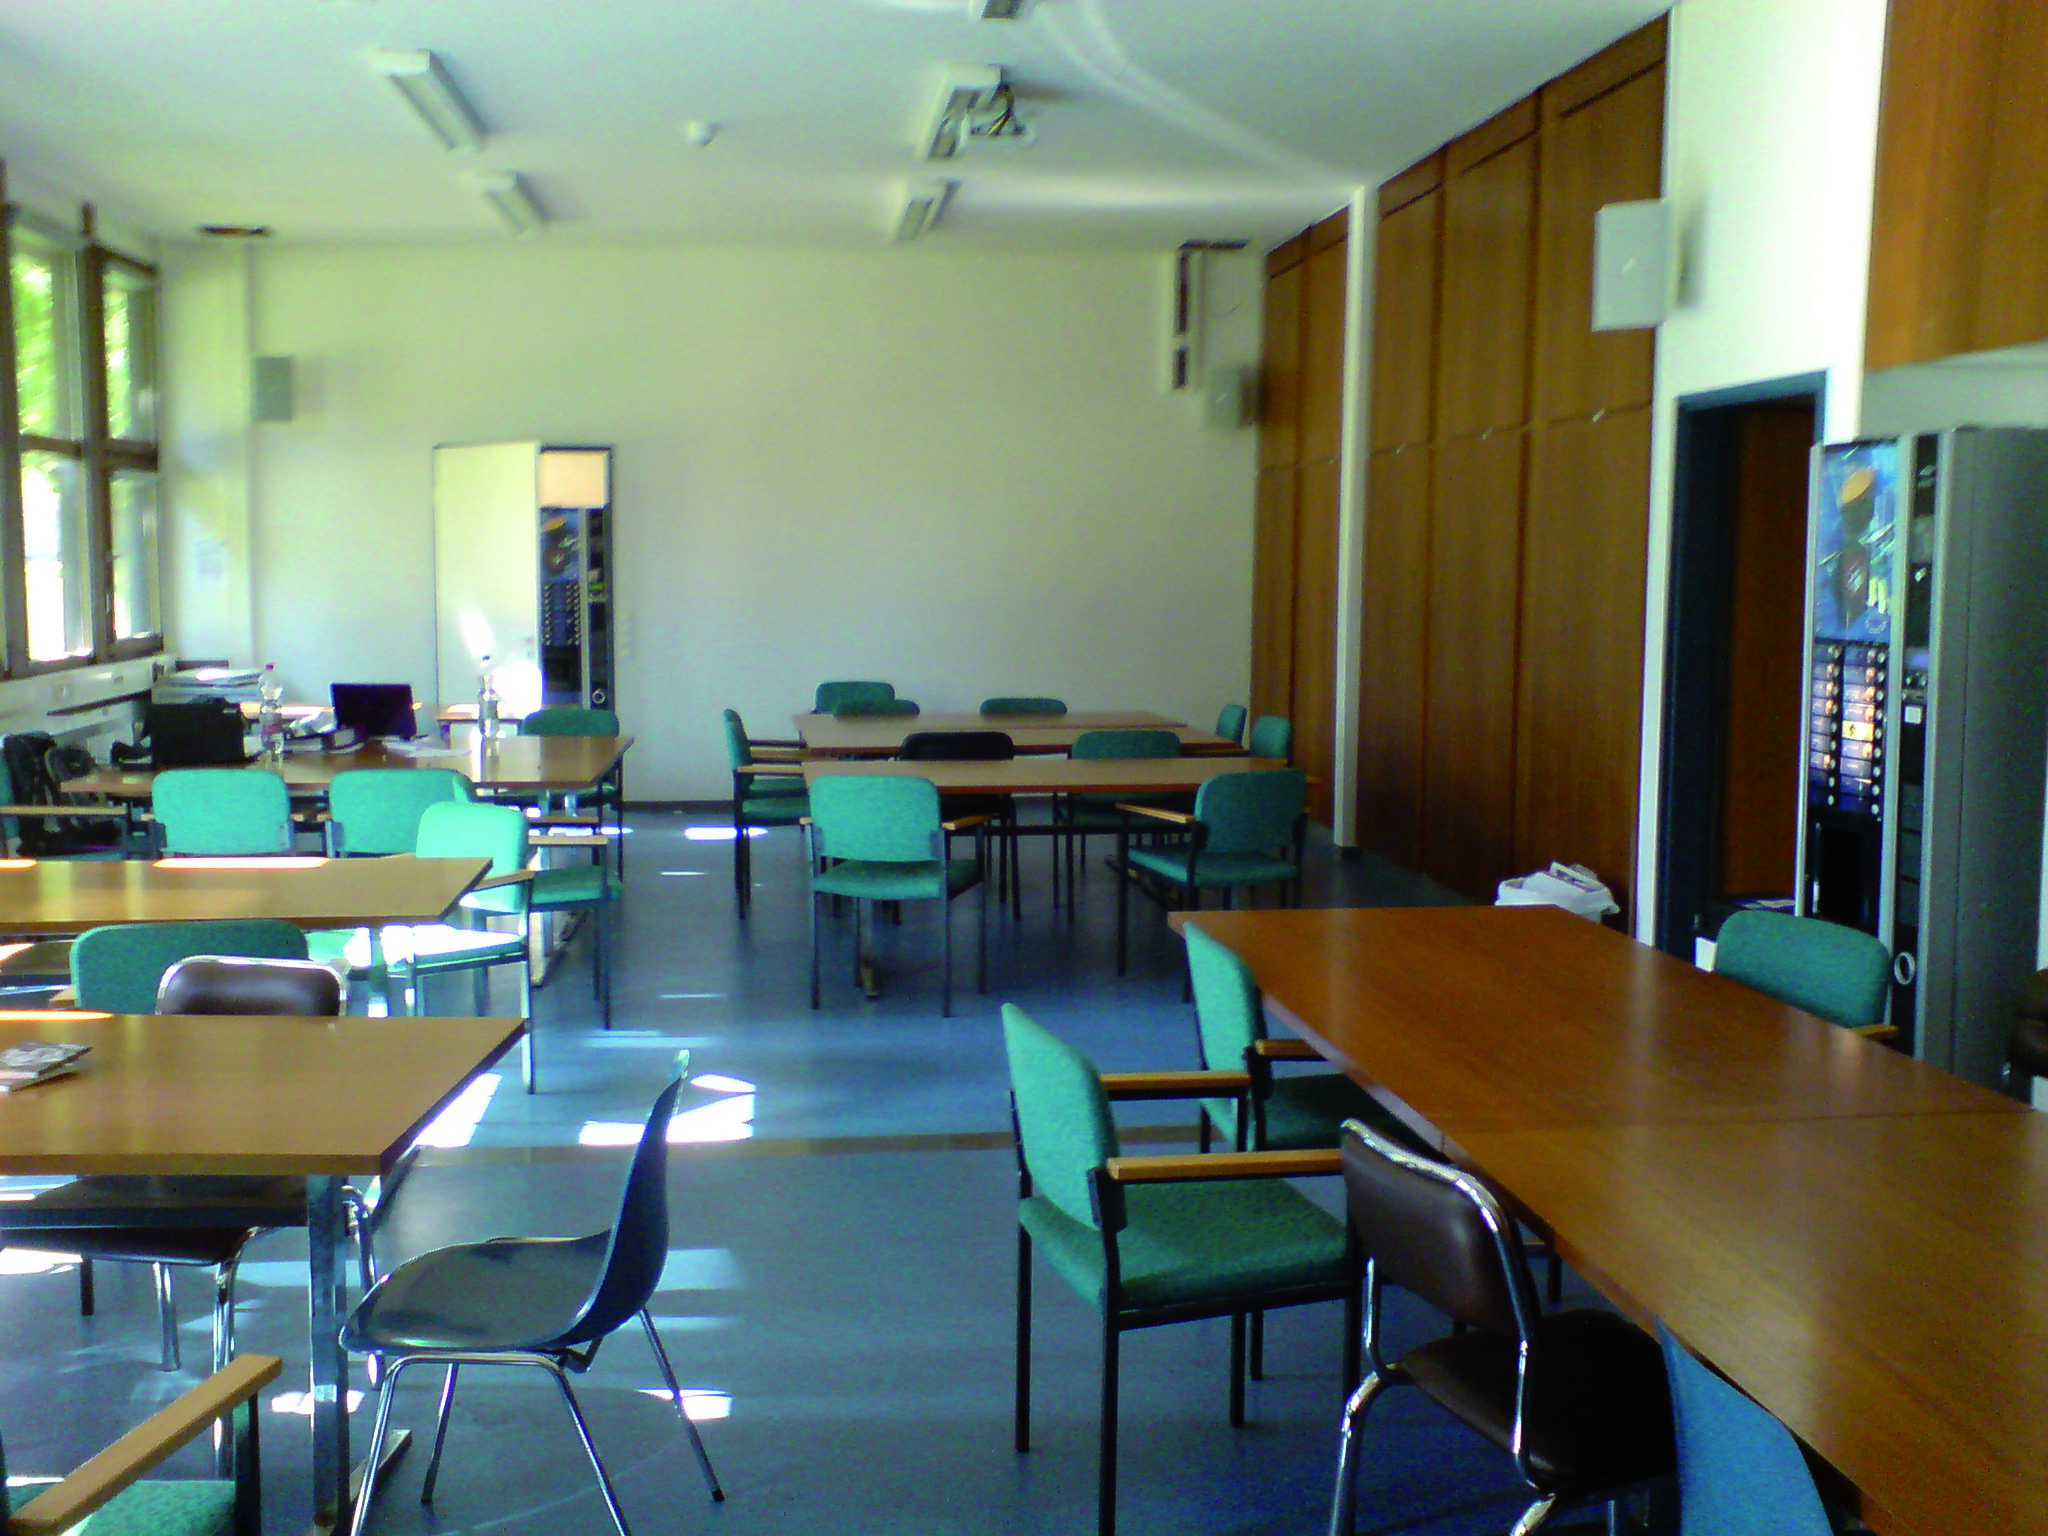
\includegraphics[width=\textwidth]{gumbel_raum_print}
